% Reflexiones, isometrías y similaridades (partición de 03-reflexiones-afinidades-homogeneas.tex, fase B)
\chapter{Reflexiones, isometrías y similaridades}\label{cap:reflexiones}\label{sec:bloque-euclideas}

\section{La idea}

Reflejamos y escalamos. Con reflexiones se construyen rotaciones, y con una escala común se pasa a las similaridades. Seguimos el hilo de la construcción: reflexiones, rotaciones, escalas.

\subsection{Reflejar y componer}\label{sec:reflejar}

\unidadInteractiva{03_reflexiones_similaridades}{Reflexiones y similaridades}{Explorá: elegí el caso «espejo de la recta de ángulo \(\alpha\)», mové \(\alpha\) y mirá cómo el área con signo de la parcela cambia de signo mientras las distancias no cambian.}

Una reflexión invierte una figura respecto de un centro o de una recta. Aplicada dos veces
respecto del mismo elemento devuelve la figura original. Esta propiedad se llama involución.

La riqueza geométrica aparece al combinar reflexiones distintas:
\begin{itemize}
  \item dos reflexiones puntuales producen una traslación;
  \item dos reflexiones en rectas paralelas producen una traslación perpendicular a ellas;
  \item dos reflexiones en rectas secantes producen una rotación alrededor de su intersección;
  \item tres reflexiones puntuales vuelven a producir una reflexión puntual y construyen un
  paralelogramo.
\end{itemize}

\paragraph{Primera traducción algebraica.}
\[
  \rho_b(x)=2b-x.
\]
La diferencia \(\rho_b(x)-b=-(x-b)\) indica que la imagen conserva la distancia a \(b\),
pero queda en la dirección opuesta. Al componer dos reflexiones, los términos que dependen de
\(x\) recuperan su signo y queda un desplazamiento constante.

\begin{idea}[Una reflexión invierte la orientación; dos la restituyen]
Cada reflexión individual cambia la orientación. Dos reflexiones vuelven a preservarla. La
posición relativa de los centros o de los ejes decide si el resultado se interpreta como
traslación o como rotación.
\end{idea}

\begin{idea}[Dos reflexiones sucesivas componen una rotación]
Con reflexiones se pueden construir rotaciones: un par de reflexiones sucesivas no altera
las distancias pero tiene un punto fijo, así que tiene que ser una rotación.
\end{idea}

\subsection{Escalar: homotecias y similaridades}\label{sec:escalar}

Una homotecia cambia el tamaño respecto de un centro. Cada punto permanece sobre la recta que
lo une con ese centro. Si la razón es positiva conserva el semirayo; si es negativa pasa al
semirayo opuesto.

Una similaridad combina escala uniforme, giro y, eventualmente, reflexión o traslación. La
figura puede cambiar de tamaño y posición, pero conserva sus ángulos y sus proporciones. Dos
triángulos relacionados por una similaridad tienen la misma forma.

\paragraph{Primera traducción algebraica.}
\[
  x'=o+k(x-o).
\]
El término \(x-o\) mira el punto desde el centro. Multiplicarlo por \(k\) cambia su distancia
y, si \(k<0\), también invierte el semirayo.

\begin{idea}[La escala es un múltiplo de la identidad]
Así como la rotación se expresa en complejos también se expresa la escala, que en
matrices se representa con una matriz múltiplo de la identidad.
\end{idea}

\section{Construcciones, cuentas y ejemplos}

Este nivel es la guía de transformaciones. Reproducimos los enunciados de \texttt{Ejercicios.pdf}, y resolvemos cada definición y cada teorema de dos maneras, con una construcción y con un ejemplo con vectores. La resolución es desarrollo nuestro.

\subsection{Enunciados originales de la guía}

Los textos siguientes reproducen los enunciados de \texttt{Ejercicios.pdf}. Se normalizaron
únicamente los cortes de línea, la notación matemática y errores tipográficos evidentes; las
dos páginas originales se incluyen completas como anexo facsimilar al final del documento.

\begin{enunciado}[Definición 1]
La reflexión del punto \(a\) por un punto \(b\) es la operación que lleva el punto \(a\) al
punto que está sobre la recta \(\overline{ab}\), a la misma distancia de \(b\) que \(a\),
pero al otro lado de \(b\). Se llama \(\rho_b(a)\).
\end{enunciado}

\begin{enunciado}[Teorema 1]
\(\rho_a\rho_b\), la composición de dos reflexiones, es una traslación. Puede ser expresada
algebraicamente con la suma de un vector constante o geométricamente como el desplazamiento
según un segmento fijo.
\end{enunciado}

\begin{enunciado}[Teorema 2]
Si \(\rho_d=\rho_a\rho_b\rho_c\), entonces el polígono \(abcda\) es un paralelogramo.
\end{enunciado}

\begin{enunciado}[Observación]
Con esta operación puede definirse la suma y resta de vectores. ¿De qué modo? ¿Cómo se
relaciona esto con la propiedad de que sea inversiva la transformación, es decir, que al
aplicarla dos veces se anula?
\end{enunciado}

\begin{enunciado}[Definición 2]
La reflexión del punto \(a\) por la recta \(B\), \(\varphi_B(a)\), es la operación que lleva
el punto \(a\) al punto que está sobre la perpendicular a \(B\) que pasa por \(a\), a la misma
distancia que \(a\) de \(B\), pero al otro lado de la recta \(B\).
\end{enunciado}

\begin{enunciado}[Teorema 3]
Si \(\Theta_{AB}=\varphi_A\varphi_B\) y \(A\) es paralela a \(B\), entonces
\(\Theta_{AB}\) es una traslación. Puede ser expresada algebraicamente con la suma de un
vector constante o geométricamente como el desplazamiento según un segmento fijo.
\end{enunciado}

\begin{enunciado}[Teorema 4]
Si \(\Theta_{AB}=\varphi_A\varphi_B\) y \(A\) no es paralela a \(B\), entonces
\(\Theta_{AB}\) es una rotación.
\end{enunciado}

\begin{enunciado}[Teorema 5]
Si \(\Theta_{ABCD}=\Theta_{AB}\Theta_{CD}\), con \(\Theta_{AB}\) una traslación y
\(\Theta_{CD}\) una rotación, entonces \(\Theta_{ABCD}\) es una rotación. Además,
\(\Theta_{CDAB}=\Theta_{CD}\Theta_{AB}\) es también una rotación, pero es distinta.
\end{enunciado}

\begin{enunciado}[Definición 3]
Una homotecia con centro en el punto \(o\) y razón \(k\), nombrada \(\eta_o^k\), lleva un
punto \(a\) a otro sobre la recta \(\overline{oa}\), de forma que
\[
  \frac{d\bigl(o,\eta_o^k(a)\bigr)}{d(o,a)}=k,
\]
donde \(d(a,b)\) es la distancia entre el punto \(a\) y el punto \(b\). Los puntos \(a\) y
\(\eta_o^k(a)\) están al mismo lado del punto \(o\) en la recta \(\overline{oa}\).
\end{enunciado}

\begin{atencion}[Precisión sobre el texto original]
La razón entre distancias es siempre no negativa. Por eso, la redacción original corresponde
al caso \(k>0\). Para una razón firmada debe escribirse
\[
\eta_o^k(a)=o+k(a-o),
\qquad
\frac{d\bigl(o,\eta_o^k(a)\bigr)}{d(o,a)}=|k|.
\]
Punto e imagen están del mismo lado de \(o\) si \(k>0\), y en lados opuestos si \(k<0\).
\end{atencion}

\begin{enunciado}[Teorema 6]
Cualquier transformación de similaridad del plano puede expresarse como la composición
\(\varphi_A\varphi_B\eta_o^k\), donde el punto \(o\) es la intersección de las rectas
\(A\) y \(B\), y es el punto fijo de la transformación. Dado un triángulo y su imagen bajo
esta transformación puede hallarse el punto \(o\) con la construcción de Euler indicada en
la guía original.
\end{enunciado}

\begin{atencion}[Alcance del Teorema 6 original]
Tal como está escrito, el enunciado es demasiado general. La composición de dos reflexiones
y una homotecia describe una similaridad directa con punto fijo. Una similaridad inversa
requiere una cantidad impar de reflexiones, y una traslación no posee punto fijo finito.
\end{atencion}

\begin{enunciado}[Ejercicios]
Para cada una de las definiciones y teoremas expuestos, verificar la conclusión con un ejemplo
gráfico y construyendo un ejemplo algebraico con vectores. Pista para las reflexiones: para
hallar la proyección perpendicular de un punto sobre una recta puede usarse el producto
interno o construir la ecuación vectorial de la perpendicular usando el vector normal que
surge de la ecuación canónica de la recta.
\end{enunciado}

\subsection{Resolución completa de la guía}

La consigna de la guía no contiene una lista de problemas independientes. Solicita verificar
\textbf{cada definición y cada teorema} de dos maneras: mediante una construcción geométrica
y mediante un ejemplo algebraico con vectores. Las secciones siguientes constituyen esa
resolución punto por punto.

\begin{center}
\begin{tabularx}{\textwidth}{>{\bfseries}p{34mm} X X}
\toprule
Ítem de la guía & Verificación geométrica & Verificación algebraica\\
\midrule
Definición 1 & punto medio y segmentos iguales & \(\rho_b(x)=2b-x\)\\
Teorema 1 & desplazamiento constante & composición de dos reflexiones puntuales\\
Teorema 2 & diagonales que se bisecan & \(d=a-b+c\)\\
Definición 2 & perpendicular y distancias iguales & proyección mediante el vector normal\\
Teorema 3 & avance perpendicular de longitud \(2h\) & composición con normales paralelos\\
Teorema 4 & ángulo final igual a \(2\theta\) & producto de matrices de reflexión\\
Teorema 5 & mismo giro, distinto centro & resolución del punto fijo\\
Definición 3 & rayos desde el centro & \(\eta_o^k(x)=o+k(x-o)\)\\
Teorema 6 & escala y giro con centro común & \(S(x)=o+\lambda R(x-o)\)\\
\bottomrule
\end{tabularx}
\end{center}

\begin{idea}[Cada ítem se resuelve con un dibujo y con una cuenta]
Cada apartado presenta el dibujo o construcción, la propiedad geométrica que debe observarse,
la demostración vectorial y un ejemplo numérico. Los ejercicios del final son práctica
adicional y no sustituyen estas soluciones.
\end{idea}

\subsection{Guía resuelta: reflexión respecto de un punto}

\subsubsection{Definición 1}

La reflexión de \(x\) respecto del punto \(b\) deja a \(b\) como punto medio del segmento
que une \(x\) con su imagen. Por lo tanto,
\[
  \frac{x+\rhoP{b}(x)}{2}=b
  \qquad\Longrightarrow\qquad
  \boxed{\rhoP{b}(x)=2b-x}.
\]

\begin{center}
\begin{tikzpicture}[scale=1.0]
  \coordinate (x) at (1,1.5);
  \coordinate (b) at (5,2.4);
  \coordinate (xp) at (9,3.3);
  \draw[auxline] (.4,1.36)--(9.6,3.44);
  \draw[decorate,decoration={brace,amplitude=5pt,mirror},teal]
    (x)--node[below=5pt,font=\small] {$d(x,b)$}(b);
  \draw[decorate,decoration={brace,amplitude=5pt,mirror},teal]
    (b)--node[below=5pt,font=\small] {$d(b,\rho_b(x))$}(xp);
  \fill[teal] (x) circle (2.4pt) node[above left] {$x$};
  \fill[ink] (b) circle (2.7pt) node[above] {$b$};
  \fill[rust] (xp) circle (2.4pt) node[above right] {$\rho_b(x)$};
\end{tikzpicture}
\end{center}

\begin{resultado}[Propiedades inmediatas]
\[
  \rhoP{b}\bigl(\rhoP{b}(x)\bigr)=x,
  \qquad
  \rhoP{b}(b)=b,
  \qquad
  \rhoP{b}(x)-b=-(x-b).
\]
Es una transformación involutiva: aplicarla dos veces devuelve el punto original.
\end{resultado}

\paragraph{Ejemplo.}
Si \(b=(2,1)\) y \(x=(5,3)\), entonces
\[
  \rhoP{b}(x)=2(2,1)-(5,3)=(-1,-1).
\]
El punto medio entre \((5,3)\) y \((-1,-1)\) es efectivamente \((2,1)\).

\subsection{Guía resuelta: dos reflexiones puntuales}

\subsubsection{Teorema 1: la composición es una traslación}

Sean \(a,b\in\R^2\). Aplicando primero \(\rhoP{b}\) y luego \(\rhoP{a}\):
\[
\begin{aligned}
  \rhoP{a}\rhoP{b}(x)
  &=\rhoP{a}(2b-x)\\
  &=2a-(2b-x)\\
  &=x+2(a-b).
\end{aligned}
\]

\begin{resultado}[Conclusión]
\[
  \boxed{\rhoP{a}\rhoP{b}=T_{\,2(a-b)}}
\]
La composición desplaza todos los puntos por el mismo vector \(2(a-b)\). No posee puntos
fijos salvo el caso degenerado \(a=b\), en el cual es la identidad.
\end{resultado}

\begin{center}
\begin{tikzpicture}[scale=.92]
  \coordinate (x) at (.7,1);
  \coordinate (b) at (3,1.6);
  \coordinate (y) at (5.3,2.2);
  \coordinate (a) at (6.8,2.6);
  \coordinate (z) at (8.3,3);
  \draw[auxline] (.2,.87)--(8.8,3.13);
  \draw[mainline,-{Latex[length=2.8mm]}] (x)--(z);
  \fill[teal] (x) circle (2.4pt) node[labelback,below left] {$x$};
  \fill[ink] (b) circle (2.4pt) node[labelback,above] {$b$};
  \fill[rust] (y) circle (2.4pt) node[labelback,below] {$\rho_b(x)$};
  \fill[ink] (a) circle (2.4pt) node[labelback,above] {$a$};
  \fill[teal] (z) circle (2.4pt) node[labelback,above right] {$\rho_a\rho_b(x)$};
  \node[labelback,font=\small,text=tealdark,above=16pt] at ($(x)!.5!(z)$)
    {mismo desplazamiento para cualquier \(x\)};
\end{tikzpicture}
\end{center}

\paragraph{Ejemplo.}
Con \(a=(3,2)\) y \(b=(1,1)\), la traslación resultante tiene vector
\[
  2(a-b)=2(2,1)=(4,2).
\]
Para \(x=(2,-1)\): \(\rhoP{b}(x)=(0,3)\) y
\(\rhoP{a}(0,3)=(6,1)=x+(4,2)\).

\subsection{Guía resuelta: tres reflexiones puntuales}

\subsubsection{Teorema 2: aparece un paralelogramo}

La composición de tres reflexiones puntuales vuelve a ser una reflexión puntual:
\[
\begin{aligned}
\rhoP{a}\rhoP{b}\rhoP{c}(x)
  &=2a-\bigl(2b-(2c-x)\bigr)\\
  &=2(a-b+c)-x.
\end{aligned}
\]
Si \(\rhoP{d}=\rhoP{a}\rhoP{b}\rhoP{c}\), entonces
\[
  \boxed{d=a-b+c}.
\]
Al reordenar:
\[
  a+c=b+d.
\]
Esta es precisamente la condición vectorial para que las diagonales del cuadrilátero
\(a b c d\) tengan el mismo punto medio.

\begin{center}
\begin{tikzpicture}[scale=1.0]
  \coordinate (a) at (1,1);
  \coordinate (b) at (5,1.2);
  \coordinate (c) at (7.2,4);
  \coordinate (d) at (3.2,3.8);
  \draw[mainline] (a)--(b)--(c)--(d)--cycle;
  \draw[auxline] (a)--(c);
  \draw[auxline] (b)--(d);
  \fill[teal] (a) circle (2.4pt) node[below left] {$a$};
  \fill[teal] (b) circle (2.4pt) node[below right] {$b$};
  \fill[rust] (c) circle (2.4pt) node[above right] {$c$};
  \fill[rust] (d) circle (2.4pt) node[above left] {$d=a-b+c$};
  \fill[ink] (4.1,2.5) circle (2pt);
  \node[labelback,font=\small] at (4.15,2.02) {punto medio común};
  \draw[-{Latex[length=2.2mm]},rust,line width=.8pt] (a)--(b);
  \draw[-{Latex[length=2.2mm]},rust,line width=.8pt] (d)--(c);
\end{tikzpicture}
\end{center}

\paragraph{Ejemplo.}
Si \(a=(1,1)\), \(b=(4,1)\) y \(c=(6,3)\), entonces
\[
  d=(1,1)-(4,1)+(6,3)=(3,3).
\]
Se verifica \(a+c=(7,4)=b+d\); por lo tanto, las diagonales se bisecan.

\begin{idea}[Las reflexiones puntuales suman y restan vectores]
La fórmula \(d=a-b+c\) permite construir geométricamente la operación
\(a+c-b\). Elegido un origen \(b\), el punto \(d\) representa la suma de los
vectores \(\overrightarrow{ba}+\overrightarrow{bc}\).

La suma \(u+v\) se obtiene llevando ambos vectores a un origen común y completando el
paralelogramo. La resta \(u-v\) se interpreta como \(u+(-v)\), donde \(-v\) surge de reflejar
el extremo de \(v\) respecto de su origen. Esto se relaciona con la involución porque
\[
  \rho_b^2=\operatorname{Id};
\]
reflejar dos veces no ``anula'' el punto, sino que devuelve exactamente la posición inicial.
\end{idea}

\subsection{Guía resuelta: reflexión respecto de una recta}

\subsubsection{Definición 2 y fórmula con proyección}

Sea la recta
\[
  B=\{x\in\R^2:n\cdot x=c\},
\]
donde \(n\neq0\) es un vector normal. La proyección ortogonal de \(x\) sobre \(B\) es
\[
  p=x-\frac{n\cdot x-c}{\lVert n\rVert^2}\,n.
\]
Como \(p\) debe ser el punto medio entre \(x\) y su reflejo:
\[
  \boxed{\refl{B}(x)=2p-x
  =x-2\frac{n\cdot x-c}{\lVert n\rVert^2}\,n}.
\]

\begin{center}
\begin{tikzpicture}[scale=1.0]
  \coordinate (x) at (2,4.4);
  \coordinate (p) at (4.8,2.4);
  \coordinate (xp) at (7.6,.4);
  \draw[rust,line width=1.1pt] (.4,.45)--(8.8,3.95)
    node[right,font=\small] {$B$};
  \draw[auxline] (x)--(xp);
  \draw[mainline] ($(p)+(-.32,.15)$)--($(p)+(-.17,.47)$)--($(p)+(.15,.32)$);
  \fill[teal] (x) circle (2.5pt) node[above left] {$x$};
  \fill[ink] (p) circle (2.4pt) node[above right] {$p$};
  \fill[rust] (xp) circle (2.5pt) node[below right] {$\varphi_B(x)$};
  \draw[decorate,decoration={brace,amplitude=5pt},teal]
    (x)--node[left=5pt,font=\small] {$d$}(p);
  \draw[decorate,decoration={brace,amplitude=5pt},teal]
    (p)--node[left=5pt,font=\small] {$d$}(xp);
\end{tikzpicture}
\end{center}

\paragraph{Ejemplo.}
Para \(B:\ x+2y=4\), \(n=(1,2)\) y \(x_0=(4,3)\):
\[
  n\cdot x_0-c=6,\qquad \lVert n\rVert^2=5,
\]
\[
  \refl{B}(x_0)
  =(4,3)-\frac{12}{5}(1,2)
  =\left(\frac85,-\frac95\right).
\]
La proyección es
\[
  p=(4,3)-\frac65(1,2)
  =\left(\frac{14}{5},\frac35\right).
\]
Además,
\[
  x_0-p=p-\refl{B}(x_0)=\frac65(1,2),
\]
lo que verifica simultáneamente que ambos segmentos tienen la misma longitud y que son
perpendiculares a la recta, pues son paralelos al normal \(n=(1,2)\).

\begin{ejemplo}[Reflexión respecto de la recta que pasa por dos puntos]\label{ej:reflexion-dos-puntos}
Reflejamos \(X=(5,8)\) respecto de la recta \(L\) que pasa por \(P=(1,2)\) y \(Q=(7,5)\).

\emph{Ecuación de la recta.} La dirección es \(d=Q-P=(6,3)=3\,(2,1)\), y un vector
perpendicular a \((2,1)\) es \(n=(1,-2)\). Con \(c=n\cdot P=1-4=-3\) queda
\[
  L:\ x-2y=-3 ,
\]
y \(Q\) la verifica: \(7-10=-3\).

\emph{Proyección.} Con la fórmula de la normal, \(n\cdot X-c=5-16+3=-8\) y
\(\lVert n\rVert^2=5\), así que
\[
  p=X-\frac{-8}{5}\,n=(5,8)+\frac85(1,-2)=(6{,}6;\ 4{,}8).
\]
El mismo punto sale proyectando \(X-P=(4,6)\) sobre la dirección:
\(t=\dfrac{(X-P)\cdot d}{\lVert d\rVert^2}=\dfrac{42}{45}=\dfrac{14}{15}\) y
\(p=P+t\,d=(1,2)+(5{,}6;\ 2{,}8)=(6{,}6;\ 4{,}8)\).

\emph{Reflejo.} Como \(p\) es el punto medio entre \(X\) y su imagen,
\[
  \refl{L}(X)=2p-X=(8{,}2;\ 1{,}6).
\]

\emph{Forma matricial.} Desarrollando \(\refl{L}(x)=x-2\frac{n\cdot x-c}{\lVert n\rVert^2}\,n\)
se separa una parte lineal y una traslación:
\[
  \refl{L}(x)=Hx+t,\qquad
  H=I-\frac{2\,nn^T}{\lVert n\rVert^2}=\frac15\begin{pmatrix}3&4\\4&-3\end{pmatrix},\qquad
  t=\frac{2c}{\lVert n\rVert^2}\,n=(-1{,}2;\ 2{,}4).
\]
Para \(X\): \(HX=\frac15(47,-4)=(9{,}4;\ -0{,}8)\) y \(HX+t=(8{,}2;\ 1{,}6)\). Además
\(\det H=-1\): la reflexión invierte la orientación.

\emph{Control.} \(P\) y \(Q\) están en el eje, de modo que quedan fijos y las distancias a ellos se
conservan: \(\lVert X-P\rVert^2=4^2+6^2=52\) y
\(\lVert \refl{L}(X)-P\rVert^2=7{,}2^2+0{,}4^2=52\);
\(\lVert X-Q\rVert^2=2^2+3^2=13\) y
\(\lVert \refl{L}(X)-Q\rVert^2=1{,}2^2+3{,}4^2=13\).
\end{ejemplo}

\subsection{Guía resuelta: reflexiones en rectas paralelas}

\subsubsection{Teorema 3: la composición es una traslación}\label{teo:traslacion-dos-reflexiones}

Tomemos rectas paralelas con un normal unitario \(n\):
\[
  A:\ n\cdot x=\alpha,
  \qquad
  B:\ n\cdot x=\beta.
\]
Sus reflexiones son
\[
  \refl{A}(x)=x-2(n\cdot x-\alpha)n,
  \qquad
  \refl{B}(x)=x-2(n\cdot x-\beta)n.
\]
Al componer:
\[
  \boxed{\refl{A}\refl{B}(x)=x+2(\alpha-\beta)n}.
\]

\begin{center}
\begin{tikzpicture}[scale=.94]
  \draw[rust,line width=1.1pt] (1,.5)--(1,5) node[above] {$B$};
  \draw[rust,line width=1.1pt] (4,.5)--(4,5) node[above] {$A$};
  \coordinate (x) at (0,1.2);
  \coordinate (y) at (2,1.2);
  \coordinate (z) at (6,1.2);
  \draw[auxline] (x)--(z);
  \draw[mainline,-{Latex[length=2.8mm]}] (x)--(z);
  \fill[teal] (x) circle (2.5pt) node[below] {$x$};
  \fill[rust] (y) circle (2.5pt) node[below] {$\varphi_B(x)$};
  \fill[teal] (z) circle (2.5pt) node[below] {$\varphi_A\varphi_B(x)$};
  \draw[<->,muted] (1,4.1)--node[above,font=\small] {$h$}(4,4.1);
  \node[font=\small,text=tealdark] at (3,2.3) {desplazamiento \(2h\)};
\end{tikzpicture}
\end{center}

\paragraph{Lectura geométrica.}
La primera reflexión cruza \(B\); la segunda cruza \(A\). El desplazamiento total es
perpendicular a ambas rectas y su módulo es dos veces la distancia entre ellas. Invertir el
orden invierte el vector de traslación.

\paragraph{Ejemplo gráfico y algebraico común.}
Si \(B:x=1\), \(A:x=4\) y \(p=(0,2)\), entonces
\[
  p=(0,2)
  \xmapsto{\ \refl{B}\ }(2,2)
  \xmapsto{\ \refl{A}\ }(6,2).
\]
Por tanto,
\[
  \refl{A}\refl{B}(x,y)=(x+6,y).
\]
La distancia entre los ejes es \(3\), la traslación tiene módulo \(6\) y el punto intermedio
\((2,2)\) muestra las dos reflexiones separadamente.

\subsection{Guía resuelta: reflexiones en rectas secantes}

\subsubsection{Teorema 4: la composición es una rotación}\label{teo:rotacion-dos-reflexiones}

Sean \(A\) y \(B\) dos rectas que se cortan en \(o\), formando un ángulo orientado
\(\theta\) desde \(B\) hasta \(A\). Como ambas reflexiones fijan \(o\), su composición
también lo fija. Además, cada reflexión invierte orientación; dos reflexiones la preservan.
El efecto angular total es
\[
  \boxed{\refl{A}\refl{B}=R_{o,\,2\theta}}.
\]

\begin{center}
\begin{tikzpicture}[scale=1.0]
  \coordinate (o) at (4,2.2);
  \coordinate (x) at (7.4,1.35);
  \coordinate (y) at (6.5,4.1);
  \draw[rust,line width=1.05pt] (.4,2.2)--(8,2.2) node[right] {$B$};
  \draw[rust,line width=1.05pt] ($(o)+(-3,-1.73)$)--($(o)+(3,1.73)$)
    node[right] {$A$};
  \draw[auxline] (o)--(x);
  \draw[auxline] (o)--(y);
  \draw[mainline,-{Latex[length=2.6mm]}] (x) arc[start angle=-14,end angle=39,
    radius=3.5];
  \fill[ink] (o) circle (2.6pt) node[below left] {$o$};
  \fill[teal] (x) circle (2.5pt) node[below right] {$x$};
  \fill[teal] (y) circle (2.5pt)
    node[labelback,above right=2pt] {$\varphi_A\varphi_B(x)$};
  \draw[teal,line width=.7pt] ($(o)+(.9,0)$)
    arc[start angle=0,end angle=30,radius=.9];
  \node[labelback,font=\small,text=teal] at ($(o)+(1.15,.32)$) {$\theta$};
  \node[labelback,font=\small,text=tealdark] at (6.05,2.86) {giro total \(2\theta\)};
\end{tikzpicture}
\end{center}

\paragraph{Verificación matricial.}
Si ambas rectas pasan por el origen y \(A\) forma ángulo \(\alpha\), la matriz de reflexión es
\[
  H(\alpha)=
  \begin{pmatrix}
    \cos 2\alpha & \sin 2\alpha\\
    \sin 2\alpha &-\cos 2\alpha
  \end{pmatrix}.
\]
Por multiplicación directa,
\[
  H(\alpha)H(\beta)=
  \begin{pmatrix}
    \cos 2(\alpha-\beta)&-\sin 2(\alpha-\beta)\\
    \sin 2(\alpha-\beta)& \cos 2(\alpha-\beta)
  \end{pmatrix}
  =R\bigl(2(\alpha-\beta)\bigr).
\]

\paragraph{Ejemplo numérico completo.}
Sea \(B\) el eje \(x\), sea \(A\) una recta por el origen que forma \(30^\circ\) con \(B\),
y sea \(p=(1,1)\). Primero:
\[
  p_1=\varphi_B(p)=(1,-1).
\]
La reflexión respecto de \(A\) tiene matriz
\[
H(30^\circ)=
\begin{pmatrix}
\frac12&\frac{\sqrt3}{2}\\
\frac{\sqrt3}{2}&-\frac12
\end{pmatrix}.
\]
Por lo tanto,
\[
p_2=\varphi_A(p_1)
=
\begin{pmatrix}
\frac12-\frac{\sqrt3}{2}\\[1mm]
\frac{\sqrt3}{2}+\frac12
\end{pmatrix}.
\]
Este es exactamente
\[
R(60^\circ)(1,1)^T.
\]
El punto \(p\) se refleja primero debajo de \(B\) y luego cruza \(A\); el ángulo neto observado
desde el origen es el doble del ángulo entre los ejes.

\begin{idea}[Dos reflexiones producen la matriz de rotación]
Esta matriz es exactamente la matriz de rotación ya trabajada. La guía aporta ahora
una construcción geométrica: una rotación plana puede generarse con dos reflexiones en
rectas que se cortan en su centro.
\end{idea}

\begin{ejemplo}[Dos reflexiones: rotación o traslación según los ejes]\label{ej:dos-reflexiones}
Sean \(B:\ y=1\) y \(A:\ x-y=1\). Se cortan en \(o=(2,1)\); \(B\) es horizontal y \(A\) forma
\(45^\circ\) con ella, así que el Teorema~4 predice un giro de \(90^\circ\) alrededor de \(o\).

\emph{Las dos reflexiones.} Para \(B\) basta reflejar la ordenada respecto de \(1\):
\(\refl{B}(x,y)=(x,\,2-y)\). Para \(A\), con \(n=(1,-1)\), \(\lVert n\rVert^2=2\) y \(c=1\),
\[
  \refl{A}(x,y)=(x,y)-(x-y-1)(1,-1)=(y+1,\ x-1).
\]

\emph{La composición.}
\[
  \refl{A}\refl{B}(x,y)=\refl{A}(x,\,2-y)=(3-y,\ x-1).
\]
La rotación de \(90^\circ\) con centro \(o\) da lo mismo:
\(o+R(90^\circ)\bigl((x,y)-o\bigr)=(2,1)+\bigl(-(y-1),\,x-2\bigr)=(3-y,\ x-1)\).
Con \(p=(4,0)\): \(\refl{B}(p)=(4,2)\) y \(\refl{A}(4,2)=(3,3)\). Desde \(o\), los vectores
\(p-o=(2,-1)\) y \((3,3)-o=(1,2)\) miden ambos \(\sqrt5\) y son perpendiculares.

\emph{El orden.} \(\refl{B}\refl{A}(p)=\refl{B}(1,3)=(1,-1)\), que es la rotación de
\(-90^\circ\) alrededor de \(o\): \((2,1)+(-1,-2)=(1,-1)\). Invertir el orden invierte el giro.

\emph{Ejes paralelos.} Si en lugar de \(B\) se toma \(B':\ x-y=-3\), paralela a \(A\),
\[
  \refl{B'}(x,y)=(x,y)-(x-y+3)(1,-1)=(y-3,\ x+3),
  \qquad
  \refl{A}\refl{B'}(x,y)=(x+4,\ y-4).
\]
Es la traslación de vector \((4,-4)\), paralelo a \(n\) y por lo tanto perpendicular a las dos
rectas, de módulo \(4\sqrt2\approx5{,}657\): el doble de la distancia
\(\dfrac{|1-(-3)|}{\sqrt2}=2\sqrt2\approx2{,}828\) entre ellas, como afirma el Teorema~3.
Con \(p=(4,0)\): \(\refl{B'}(p)=(-3,7)\) y \(\refl{A}(-3,7)=(8,-4)=p+(4,-4)\).
\end{ejemplo}

\unidadInteractiva{03_reflexiones_similaridades}{Reflexiones y similaridades}{Verificá: elegí «dos espejos seguidos», poné \(\beta=45^\circ\) y comprobá que el resultado es \(R(90^\circ)\), con \(\det=+1\).}

\subsection{Guía resuelta: traslación y rotación}

\subsubsection{Teorema 5: el orden cambia el centro}

Sea \(T_v(x)=x+v\) y sea una rotación de parte lineal \(R\) y centro \(c\):
\[
  Q_c(x)=c+R(x-c)=Rx+(I-R)c.
\]

\paragraph*{Primero rotar, después trasladar}
\[
  T_vQ_c(x)=Rx+(I-R)c+v.
\]
Si el ángulo no es \(0\) módulo \(2\pi\), la matriz \(I-R\) es invertible y existe un único
centro \(c_1\):
\[
  \boxed{c_1=c+(I-R)^{-1}v}.
\]

\paragraph*{Primero trasladar, después rotar}
\[
  Q_cT_v(x)=Rx+(I-R)c+Rv,
\]
por lo que su centro es
\[
  \boxed{c_2=c+(I-R)^{-1}Rv}.
\]
En general \(c_1\neq c_2\): ambas composiciones tienen el mismo ángulo, pero centros distintos.

\begin{center}
\begin{tikzpicture}[scale=.92]
  \coordinate (c) at (4,2.4);
  \coordinate (c1) at (2,4.4);
  \coordinate (c2) at (6.4,4.1);
  \coordinate (x) at (5.8,1);
  \draw[auxline] (c)--(x);
  \draw[-{Latex[length=2.5mm]},teal,line width=1pt] (x) arc[start angle=-35,end angle=35,radius=2.2];
  \draw[-{Latex[length=2.5mm]},rust,line width=1pt]
    (1.3,.8)--node[labelback,below,font=\small] {$v$}(3.1,1.45);
  \fill[ink] (c) circle (2.6pt) node[labelback,below] {$c$};
  \fill[teal] (c1) circle (2.6pt) node[labelback,above left] {$c_1$};
  \fill[rust] (c2) circle (2.6pt) node[labelback,above right] {$c_2$};
  \draw[teal,dashed] (c1) circle (1.25);
  \draw[rust,dashed] (c2) circle (1.25);
  \node[labelback,font=\small,text=teal] at (1.85,3.15) {\(T_vQ_c\)};
  \node[labelback,font=\small,text=rust] at (7.05,3.0) {\(Q_cT_v\)};
\end{tikzpicture}
\end{center}

\begin{atencion}[Caso excepcional]
Si \(R=I\), no hay una rotación no trivial: las composiciones son simplemente la traslación
\(T_v\). Por eso el enunciado debe entenderse para una rotación de ángulo no nulo.
\end{atencion}

\paragraph{Ejemplo de orden.}
Sea \(R\) el giro de \(90^\circ\) alrededor del origen y \(v=(2,0)\). Entonces
\[
  T_vR(x)=Rx+(2,0),
  \qquad
  RT_v(x)=Rx+(0,2).
\]
El centro del primero es \((1,1)\); el del segundo es \((-1,1)\). El ángulo es el mismo,
pero las transformaciones son distintas.

Siguiendo el mismo punto \(p=(1,0)\):
\[
p\xmapsto{\ R\ }(0,1)
\xmapsto{\ T_v\ }(2,1),
\]
mientras que
\[
p\xmapsto{\ T_v\ }(3,0)
\xmapsto{\ R\ }(0,3).
\]
La separación entre \((2,1)\) y \((0,3)\) permite ver directamente que el orden cambió la
transformación.

\subsection{Guía resuelta: homotecia}

\subsubsection{Definición 3}

La homotecia de centro \(o\) y razón \(k\) se escribe
\[
  \boxed{\homot{o}{k}(x)=o+k(x-o)=kx+(1-k)o}.
\]

\begin{center}
\begin{tikzpicture}[scale=.95]
  \coordinate (o) at (1,1);
  \coordinate (a) at (4,2.2);
  \coordinate (ap) at (7,3.4);
  \draw[auxline] (.5,.8)--(8,3.8);
  \draw[mainline,-{Latex[length=2.6mm]}] (a)--(ap);
  \fill[ink] (o) circle (2.6pt) node[below left] {$o$};
  \fill[teal] (a) circle (2.6pt) node[above left] {$a$};
  \fill[rust] (ap) circle (2.6pt) node[above right] {$\eta_o^k(a)$};
  \draw[decorate,decoration={brace,amplitude=5pt,mirror},teal]
    (o)--node[below=5pt,font=\small] {$r$}(a);
  \draw[decorate,decoration={brace,amplitude=5pt,mirror},rust]
    (o)--node[below=5pt,font=\small] {$kr$}(ap);
\end{tikzpicture}
\end{center}

\begin{center}
\begin{tabularx}{.92\textwidth}{>{\bfseries}c X}
\toprule
Valor de \(k\) & Efecto geométrico\\
\midrule
\(k>1\) & ampliación; imagen y punto están del mismo lado de \(o\)\\
\(0<k<1\) & reducción; imagen entre \(o\) y el punto\\
\(k=1\) & identidad\\
\(k=0\) & todos los puntos colapsan en \(o\); no es una similaridad invertible\\
\(k<0\) & escala por \(|k|\) y cambia al semirayo opuesto\\
\bottomrule
\end{tabularx}
\end{center}

\paragraph{Ejemplo.}
Con \(o=(1,1)\), \(k=2\) y \(a=(3,2)\):
\[
  \homot{o}{2}(a)=(1,1)+2(2,1)=(5,3).
\]
La distancia al centro se duplica y la dirección desde \(o\) se conserva.

\subsection{Guía resuelta: similaridades}

\subsubsection{Teorema 6}

Una similaridad conserva ángulos y multiplica todas las distancias por un mismo factor
\(\lambda>0\). Una similaridad directa con punto fijo \(o\) tiene la forma
\[
  S(x)=o+\lambda R(x-o),
\]
donde \(R\) es una rotación. Como toda rotación plana puede expresarse como composición de
dos reflexiones en rectas que se cortan en \(o\),
\[
  \boxed{S=\refl{A}\refl{B}\homot{o}{\lambda}}.
\]
La homotecia conmuta con las reflexiones cuyos ejes pasan por \(o\), porque todas actúan
sobre el vector \(x-o\).

\begin{center}
\begin{tikzpicture}[scale=.88]
  \coordinate (o) at (1.3,1.1);
  \coordinate (a) at (3.1,1.4);
  \coordinate (b) at (2.2,3);
  \coordinate (c) at (4,2.7);
  \coordinate (ap) at (6.2,2.1);
  \coordinate (bp) at (5.7,5.0);
  \coordinate (cp) at (8.6,4.3);
  \draw[teal,line width=1.1pt] (a)--(b)--(c)--cycle;
  \draw[rust,line width=1.1pt] (ap)--(bp)--(cp)--cycle;
  \draw[auxline] (o)--(a);
  \draw[auxline] (o)--(ap);
  \fill[ink] (o) circle (2.7pt) node[below left] {$o$};
  \foreach \p/\lab in {a/a,b/b,c/c}
    \fill[teal] (\p) circle (2.1pt)
      node[labelback,above left=1.5pt,font=\small] {$\lab$};
  \foreach \p/\lab in {ap/S(a),bp/S(b),cp/S(c)}
    \fill[rust] (\p) circle (2.1pt)
      node[labelback,above right=1.5pt,font=\small] {$\lab$};
  \draw[-{Latex[length=2.6mm]},tealdark,line width=.9pt] (3.9,.7)
    .. controls (4.8,.2) and (5.6,.8) .. (6.1,1.5);
  \node[font=\small,text=tealdark] at (5,.35) {escala \(+\) giro};
\end{tikzpicture}
\end{center}

\begin{atencion}[Alcance del enunciado]
La composición de dos reflexiones preserva la orientación. Por eso la fórmula anterior
describe las similaridades directas. Una similaridad inversa requiere una cantidad impar de
reflexiones, por ejemplo una reflexión y una homotecia. Si la similaridad no tiene punto fijo
finito, aparece el caso especial de una traslación o una transformación con componente de
traslación.
\end{atencion}

\begin{ejemplo}[La similaridad directa que lleva un segmento a otro]\label{ej:similaridad-segmento}
Buscamos la similaridad directa \(S\) que lleva \(P=(1,1)\) a \(P'=(-3,-1)\) y \(Q=(3,2)\) a
\(Q'=(-3,4)\). Identificamos el plano con \(\mathbb{C}\); una similaridad directa es
\(S(z)=\alpha z+\beta\), con \(\alpha=a+ib\), porque multiplicar por \(\alpha\) es girar
el ángulo de \(\alpha\) y escalar por \(\lvert\alpha\rvert\). En matrices,
\(S(x)=\left(\begin{smallmatrix}a&-b\\b&a\end{smallmatrix}\right)x+t\).

\emph{Razón y ángulo.} Restando \(S(Q)-S(P)\) desaparece \(\beta\):
\[
  \alpha=\frac{Q'-P'}{Q-P}=\frac{5i}{2+i}=\frac{5i\,(2-i)}{5}=1+2i .
\]
La razón es \(\lambda=\lvert\alpha\rvert=\sqrt5\approx2{,}236\), que coincide con
\(\lVert P'Q'\rVert/\lVert PQ\rVert=5/\sqrt5\), y el ángulo es
\(\theta=\operatorname{atan2}(2,1)\approx63{,}43^\circ\).

\emph{Traslación.} \(\beta=P'-\alpha P=(-3-i)-(1+2i)(1+i)=(-3-i)-(-1+3i)=-2-4i\), es decir
\[
  S(x,y)=(x-2y-2,\ 2x+y-4),
\]
y en efecto \(S(3,2)=(-3,4)\).

\emph{Centro.} El punto fijo cumple \(c=\alpha c+\beta\):
\[
  c=\frac{\beta}{1-\alpha}=\frac{-2-4i}{-2i}=2-i,
\]
o sea \(c=(2,-1)\); en matrices, \((I-A)c=t\) con
\(I-A=\left(\begin{smallmatrix}0&2\\-2&0\end{smallmatrix}\right)\) da lo mismo. Control:
\(\lVert P-c\rVert=\lVert(-1,2)\rVert=\sqrt5\) y \(\lVert P'-c\rVert=\lVert(-5,0)\rVert=5=\sqrt5\cdot\sqrt5\),
y el ángulo de \(P-c\) a \(P'-c\) es \(63{,}43^\circ\).

\emph{Descomposición.} Por el Teorema~6,
\(S=\refl{A}\refl{B}\homot{c}{\sqrt5}\), con dos rectas \(A\) y \(B\) por \(c=(2,-1)\) que
formen un ángulo de \(\theta/2\approx31{,}72^\circ\).
\end{ejemplo}

\section{En profundidad}

Cerramos el tema con dos complementos de la guía: un ejemplo numérico completo de la descomposición de una similaridad y el método para recuperar el centro a partir de un triángulo y su imagen. Ambos son desarrollo nuestro.

\subsection{Ejemplo numérico de la descomposición}

\begin{ejemplo}[Una similaridad de razón \(2\) y giro de \(90^\circ\) como dos reflexiones y una homotecia]\label{ej:descomposicion-similaridad}
Tomemos \(o=(0,0)\), una escala \(\lambda=2\) y una rotación de \(90^\circ\). Para el
triángulo
\[
  a=(1,0),\qquad b=(0,1),\qquad c=(1,1),
\]
la similaridad
\[
  S(x)=2R(90^\circ)x
\]
produce
\[
  a'=(0,2),\qquad b'=(-2,0),\qquad c'=(-2,2).
\]
Elija como primer eje de reflexión \(B\) el eje \(x\), y como segundo eje \(A\) la recta
\(y=x\), que forma \(45^\circ\) con \(B\). Entonces
\[
  \varphi_A\varphi_B=R(90^\circ),
\]
porque el giro resultante es el doble del ángulo entre los ejes. Finalmente, la homotecia
\(\eta_o^2\) duplica todas las distancias al origen:
\[
  \boxed{S=\varphi_A\varphi_B\eta_o^2}.
\]
Geométricamente se ven tres etapas: reflexión en \(B\), reflexión en \(A\) y expansión radial
desde \(o\).
\end{ejemplo}

\subsection{Cómo hallar el centro a partir de un triángulo y su imagen}

Supongamos que una similaridad directa lleva los vértices
\[
  a\mapsto a',\qquad b\mapsto b',\qquad c\mapsto c'.
\]
Primero se determina el factor de escala y el ángulo:
\[
  \lambda=\frac{\lVert b'-a'\rVert}{\lVert b-a\rVert},
  \qquad
  \theta=\angle\bigl(b-a,b'-a'\bigr).
\]
Con estos datos, el centro \(o\) satisface
\[
  a'=o+\lambda R(\theta)(a-o).
\]
Reordenando:
\[
  \bigl(I-\lambda R(\theta)\bigr)o
  =a'-\lambda R(\theta)a,
\]
y, cuando la matriz es invertible,
\[
  \boxed{
  o=
  \bigl(I-\lambda R(\theta)\bigr)^{-1}
  \left(a'-\lambda R(\theta)a\right)
  }.
\]
El mismo resultado debe obtenerse usando \(b\mapsto b'\) o \(c\mapsto c'\).

\paragraph{Construcción geométrica.}
Como la similaridad multiplica todas las distancias al centro por \(\lambda\),
\[
  \lVert o-a'\rVert=\lambda\lVert o-a\rVert,
  \qquad
  \lVert o-b'\rVert=\lambda\lVert o-b\rVert.
\]
El primer lugar geométrico es el círculo de Apolonio asociado al par \((a,a')\), y el segundo
es el correspondiente a \((b,b')\). Sus intersecciones proporcionan los centros candidatos.
Se elige el que verifica el ángulo orientado \(\theta\). Si \(\lambda=1\), ambos lugares se
reducen a las mediatrices de \(aa'\) y \(bb'\), como ocurre en una rotación pura.

\begin{resultado}[Verificación del Teorema 6]
El centro se obtiene como intersección de dos condiciones geométricas de razón de distancias.
Una vez hallado, todos los segmentos que parten de \(o\) se escalan por \(\lambda\) y giran
el mismo ángulo \(\theta\). Esto completa la parte constructiva y la parte algebraica pedidas
por la guía.
\end{resultado}

\subsection{Aplicación topográfica: pasar un levantamiento local al sistema oficial}\label{sec:aplicacion-helmert}

Un levantamiento con estación total suele hacerse en un sistema local arbitrario: el origen y
la orientación de los ejes \(x\), \(y\) se eligen en el terreno, por comodidad. Para integrarlo a
la cartografía hay que expresarlo en el sistema oficial, aquí coordenadas Gauss-Krüger de la
faja~5: \(E\) hacia el este y \(N\) hacia el norte, en metros. Entre los dos sistemas hay una
traslación, una rotación y, además, un factor de escala apenas distinto de \(1\), porque las
distancias medidas en el terreno no coinciden exactamente con las distancias en el plano de
la proyección. Las tres cosas juntas forman una similaridad directa (sección~\ref{sec:escalar}):
\[
  \begin{pmatrix}E\\N\end{pmatrix}
  =\begin{pmatrix}t_E\\t_N\end{pmatrix}
  +\lambda\,R(\theta)\begin{pmatrix}x\\y\end{pmatrix}.
\]

\paragraph{Cuatro parámetros lineales.} Escribiendo \(a=\lambda\cos\theta\) y
\(b=\lambda\sin\theta\), la matriz \(\lambda R(\theta)\) es
\(\left(\begin{smallmatrix}a&-b\\b&a\end{smallmatrix}\right)\) y la transformación queda
\[
  \boxed{E=a\,x-b\,y+t_E,\qquad N=b\,x+a\,y+t_N.}
\]
Las incógnitas \(a\), \(b\), \(t_E\), \(t_N\) aparecen en forma lineal, aunque \(\lambda\) y
\(\theta\) no lo hagan; una vez halladas, \(\lambda=\sqrt{a^2+b^2}\) y
\(\theta=\operatorname{atan2}(b,a)\). Es la misma cuenta del
ejemplo~\ref{ej:similaridad-segmento}: en complejos,
\(E+iN=(a+ib)(x+iy)+(t_E+i\,t_N)\). Esta transformación de cuatro parámetros se conoce como
transformación de Helmert en el plano.

\paragraph{Datos.} Dos puntos de control tienen coordenadas en ambos sistemas; de otros tres
sólo se conocen las locales.
\begin{center}
\begin{tabular}{lcc}
\toprule
punto & local \((x;\,y)\) & oficial \((E;\,N)\)\\
\midrule
\(C_1\) & \(50{,}000;\ 20{,}000\) & \(5\,432\,134{,}871;\ 6\,154\,341{,}048\)\\
\(C_2\) & \(310{,}000;\ 145{,}000\) & \(5\,432\,306{,}387;\ 6\,154\,573{,}065\)\\
\(D\) & \(180{,}000;\ 60{,}000\) & ?\\
\(F\) & \(240{,}000;\ 210{,}000\) & ?\\
\(G\) & \(70{,}000;\ 150{,}000\) & ?\\
\bottomrule
\end{tabular}
\end{center}

\paragraph{Resolución con dos puntos.} Cada punto de control aporta dos ecuaciones; con dos
puntos hay cuatro ecuaciones para cuatro incógnitas. Restando las de \(C_1\) de las de \(C_2\)
se eliminan las traslaciones:
\[
  \Delta E=a\,\Delta x-b\,\Delta y,\qquad \Delta N=b\,\Delta x+a\,\Delta y,
\]
con \(\Delta x=260\), \(\Delta y=125\), \(\Delta E=171{,}516\) y \(\Delta N=232{,}017\). Este
sistema de \(2\times2\) se resuelve multiplicando la primera por \(\Delta x\) y la segunda por
\(\Delta y\) y sumando, y combinándolas en cruz para \(b\):
\[
  a=\frac{\Delta x\,\Delta E+\Delta y\,\Delta N}{\Delta x^2+\Delta y^2}
   =\frac{73\,596{,}285}{83\,225}=0{,}884305017,
\]
\[
  b=\frac{\Delta x\,\Delta N-\Delta y\,\Delta E}{\Delta x^2+\Delta y^2}
   =\frac{38\,884{,}920}{83\,225}=0{,}467226434.
\]
Volviendo a \(C_1\):
\[
  t_E=E_1-a\,x_1+b\,y_1=5\,432\,100{,}000,\qquad
  t_N=N_1-b\,x_1-a\,y_1=6\,154\,300{,}001 .
\]
De \(a\) y \(b\) salen la escala y el giro:
\[
  \lambda=\sqrt{a^2+b^2}=1{,}0001479,\qquad
  \theta=\operatorname{atan2}(b,a)=27{,}84993^\circ .
\]
La escala excede a \(1\) en \(147{,}9\) partes por millón: cada \(100\) m locales se convierten en
unos \(100{,}015\) m oficiales. Reemplazando, \(C_1\) y \(C_2\) se reproducen al milímetro, como
debe ser: la solución con dos puntos es exacta.

\paragraph{Puntos nuevos.} Con los cuatro parámetros se transforman \(D\), \(F\) y \(G\):
\begin{center}
\begin{tabular}{lcc}
\toprule
punto & local \((x;\,y)\) & oficial \((E;\,N)\)\\
\midrule
\(D\) & \(180{,}000;\ 60{,}000\) & \(5\,432\,231{,}142;\ 6\,154\,437{,}160\)\\
\(F\) & \(240{,}000;\ 210{,}000\) & \(5\,432\,214{,}116;\ 6\,154\,597{,}839\)\\
\(G\) & \(70{,}000;\ 150{,}000\) & \(5\,432\,091{,}818;\ 6\,154\,465{,}352\)\\
\bottomrule
\end{tabular}
\end{center}

\paragraph{Lo que se conserva y lo que no.} Las distancias cambian, todas en la misma
proporción:
\begin{center}
\begin{tabular}{lccc}
\toprule
lado & local (m) & oficial (m) & cociente\\
\midrule
\(DF\) & \(161{,}555\) & \(161{,}579\) & \(1{,}0001479\)\\
\(FG\) & \(180{,}278\) & \(180{,}304\) & \(1{,}0001479\)\\
\(GD\) & \(142{,}127\) & \(142{,}148\) & \(1{,}0001479\)\\
\bottomrule
\end{tabular}
\end{center}
El cociente es \(\lambda\) en los tres lados; las diferencias, \(0{,}024\), \(0{,}027\) y
\(0{,}021\) m, crecen con la longitud del lado. El ángulo en \(F\) del triángulo \(DFG\) vale
\(48{,}75856^\circ\) en los dos sistemas. No es casualidad: para \(M=\lambda R(\theta)\),
\(Mu\cdot Mv=\lambda^2\,u\cdot v\) y \(\lVert Mu\rVert\,\lVert Mv\rVert=\lambda^2\lVert u\rVert\,\lVert v\rVert\),
así que el coseno del ángulo entre dos direcciones no cambia.

\begin{figure}[htbp]
\centering
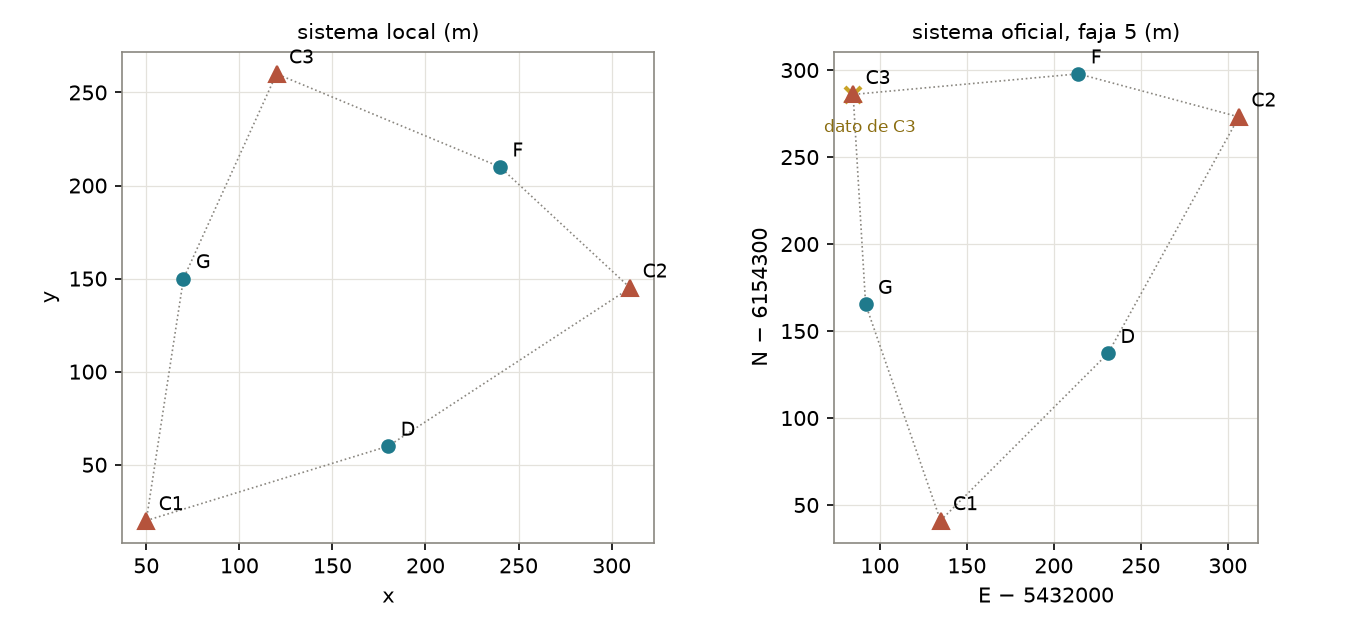
\includegraphics[width=.95\linewidth]{figuras/similaridades/helmert.png}
\caption{El levantamiento en el sistema local (izquierda) y en el oficial (derecha, con las
coordenadas referidas a un origen próximo para que se lean). Los triángulos son los puntos de
control; la cruz es el dato oficial de \(C_3\), separado de su predicción por el residuo de
\(0{,}039\) m, que a esta escala no se distingue. Generada con
\texttt{apunte/scripts/cap03\_similaridades.py}.}
\end{figure}

\paragraph{Un tercer punto de control.} Se conoce también \(C_3\), de coordenadas locales
\((120{,}000;\ 260{,}000)\) y oficiales \((5\,432\,084{,}658;\ 6\,154\,585{,}953)\). Con los
parámetros hallados, la predicción es \((5\,432\,084{,}638;\ 6\,154\,585{,}987)\), y el residuo
\[
  r=\text{dato}-\text{predicción}=(0{,}020;\ -0{,}034)\ \text{m},\qquad \lVert r\rVert=0{,}039\ \text{m}.
\]
Con tres puntos hay seis ecuaciones y cuatro incógnitas, y los datos medidos no las satisfacen
todas a la vez: ninguna similaridad lleva exactamente los tres puntos locales a los tres
oficiales. Lo confirma el cociente de distancias entre controles, que debería ser el mismo
\(\lambda\) para todos los pares y no lo es: \(1{,}0001479\) para \(C_1C_2\), \(0{,}9999984\) para
\(C_1C_3\) y \(1{,}0000492\) para \(C_2C_3\). Si se resuelve con \(C_1\) y \(C_3\) en lugar de
\(C_1\) y \(C_2\), salen otros parámetros, \(\lambda=0{,}9999984\) y \(\theta=27{,}84701^\circ\);
ahora es \(C_2\) el que no cierra, con una discrepancia de \((0{,}014;\ 0{,}043)\) m, de módulo
\(0{,}046\) m, y el punto \(D\) se corre \(0{,}021\) m. El residuo mide cuánto se apartan los
datos de una similaridad exacta: unos pocos centímetros son compatibles con errores de
medición, mientras que un residuo grande delata un punto mal identificado o mal medido.
Repartir esa discrepancia entre todos los puntos de control de la mejor manera posible es el
problema de mínimos cuadrados, que se trata en otro capítulo.

\section{Ejercicios con solución}

\subsection{Resumen de resultados}

\begin{center}
\begin{tabularx}{\textwidth}{>{\bfseries}p{31mm} X X}
\toprule
Objeto & Fórmula & Resultado clave\\
\midrule
Reflexión puntual &
\(\rho_b(x)=2b-x\) &
involución con único punto fijo \(b\)\\
Dos reflexiones puntuales &
\(\rho_a\rho_b(x)=x+2(a-b)\) &
traslación\\
Tres reflexiones puntuales &
\(\rho_a\rho_b\rho_c=\rho_d,\ d=a-b+c\) &
\(a,b,c,d\) forman paralelogramo\\
Reflexión en recta &
\(\varphi_B(x)=x-2\frac{n\cdot x-c}{\|n\|^2}n\) &
el eje queda fijo\\
Ejes paralelos &
\(\varphi_A\varphi_B(x)=x+2(\alpha-\beta)n\) &
traslación perpendicular\\
Ejes secantes &
\(\varphi_A\varphi_B=R_{o,2\theta}\) &
rotación alrededor de la intersección\\
Traslación y rotación &
\(T_vQ_c\neq Q_cT_v\) en general &
mismo ángulo, centros distintos\\
Homotecia &
\(\eta_o^k(x)=o+k(x-o)\) &
distancias multiplicadas por \(|k|\)\\
Similaridad directa &
\(S=\varphi_A\varphi_B\eta_o^\lambda\) &
escala y rotación con centro fijo\\
Helmert en el plano &
\(E=ax-by+t_E,\ N=bx+ay+t_N\) &
\(\lambda=\sqrt{a^2+b^2}\), \(\theta=\operatorname{atan2}(b,a)\)\\
\bottomrule
\end{tabularx}
\end{center}

\subsection{Ejercicios}

\begin{ejercicio}\label{ex:refl-dos-puntuales}
Sean \(a=(2,-1)\), \(b=(-1,2)\) y \(x=(4,3)\). Calcular \(\rho_a\rho_b(x)\) paso a paso y
verificar que coincide con \(x+2(a-b)\). Dibujar los cinco puntos relevantes.
\end{ejercicio}
\solucion{\(\rho_b(4,3)=2(-1,2)-(4,3)=(-6,1)\) y \(\rho_a(-6,1)=2(2,-1)-(-6,1)=(10,-3)\).
Como \(2(a-b)=(6,-6)\), también \((4,3)+(6,-6)=(10,-3)\). En el dibujo, \(b\) es el punto
medio entre \(x\) y \((-6,1)\), y \(a\) el punto medio entre \((-6,1)\) y \((10,-3)\).}

\begin{ejercicio}\label{ex:refl-paralelogramo}
Dados \(a=(1,0)\), \(b=(3,1)\) y \(c=(5,4)\), construir \(d=a-b+c\). Verificar con vectores
que \(abcd\) es un paralelogramo.
\end{ejercicio}
\solucion{\(d=a-b+c=(3,3)\). Se verifica \(b-a=c-d=(2,1)\) y \(c-b=d-a=(2,3)\): los lados
opuestos son iguales y paralelos.}

\begin{ejercicio}\label{ex:refl-recta}
Reflejar \(x=(3,4)\) respecto de \(B:\ 2x-y=1\) usando (a) la fórmula con el vector normal;
(b) la proyección perpendicular; (c) una construcción gráfica.
\end{ejercicio}
\solucion{Con \(n=(2,-1)\), \(\lVert n\rVert^2=5\) y \(n\cdot(3,4)-1=1\): (a)
\(\refl{B}(3,4)=(3,4)-\frac25(2,-1)=\left(\frac{11}{5},\frac{22}{5}\right)=(2{,}2;\ 4{,}4)\).
(b) La proyección es \(p=(3,4)-\frac15(2,-1)=\left(\frac{13}{5},\frac{21}{5}\right)=(2{,}6;\ 4{,}2)\),
y \(2p-x\) da el mismo reflejo. (c) Se traza por \(x\) la perpendicular a \(B\) (dirección
\(n\)), se marca su pie \(p\) y se lleva del otro lado la misma distancia
\(\lVert x-p\rVert=1/\sqrt5\).}

\begin{ejercicio}\label{ex:refl-ejes-paralelos}
Componer las reflexiones respecto de \(B:\ y=0\) y \(A:\ y=3\). Repetir invirtiendo el orden y
comparar los vectores de traslación.
\end{ejercicio}
\solucion{\(\refl{A}\refl{B}(x,y)=(x,\,y+6)\) y \(\refl{B}\refl{A}(x,y)=(x,\,y-6)\). Ambas son
traslaciones perpendiculares a los ejes, de módulo \(6\), el doble de la distancia entre ellos;
el orden invierte el sentido.}

\begin{ejercicio}\label{ex:refl-30}
Tomar dos rectas por el origen que formen \(30^\circ\). Multiplicar sus matrices de reflexión y
comprobar que resulta una rotación de \(60^\circ\).
\end{ejercicio}
\solucion{Con \(B\) el eje \(x\) y \(A\) a \(30^\circ\):
\(H(30^\circ)H(0^\circ)=
\left(\begin{smallmatrix}\frac12&\frac{\sqrt3}{2}\\\frac{\sqrt3}{2}&-\frac12\end{smallmatrix}\right)
\left(\begin{smallmatrix}1&0\\0&-1\end{smallmatrix}\right)
=\left(\begin{smallmatrix}\frac12&-\frac{\sqrt3}{2}\\\frac{\sqrt3}{2}&\frac12\end{smallmatrix}\right)
=R(60^\circ)\), es decir \(\left(\begin{smallmatrix}0{,}5&-0{,}866\\0{,}866&0{,}5\end{smallmatrix}\right)\).}

\begin{ejercicio}\label{ex:traslacion-rotacion}
Para \(R=R(90^\circ)\) y \(v=(1,2)\), escribir \(T_vR\) y \(RT_v\). Hallar el punto fijo de cada
una resolviendo \((I-R)c=t\).
\end{ejercicio}
\solucion{\(T_vR(x)=Rx+(1,2)\) y \(RT_v(x)=Rx+Rv=Rx+(-2,1)\). Con
\(I-R=\left(\begin{smallmatrix}1&1\\-1&1\end{smallmatrix}\right)\), los centros son
\(c_1=\left(-\frac12,\frac32\right)\) y \(c_2=\left(-\frac32,-\frac12\right)\): mismo giro,
centros distintos.}

\begin{ejercicio}\label{ex:homotecia-triangulo}
Dibujar un triángulo y aplicarle una homotecia de centro exterior con \(k=\frac32\). Comprobar
que las longitudes se multiplican por \(\frac32\) y que los lados correspondientes son
paralelos.
\end{ejercicio}
\solucion{Una elección concreta es \(o=(4,4)\), \(A=(0,0)\), \(B=(2,0)\), \(C=(0,2)\). Con
\(\homot{o}{3/2}(x)=o+\frac32(x-o)\): \(A'=(-2,-2)\), \(B'=(1,-2)\), \(C'=(-2,1)\). Los catetos
pasan de longitud \(2\) a \(3\), y \(B'-A'=\frac32(B-A)\), \(C'-A'=\frac32(C-A)\): lados
paralelos.}

\begin{ejercicio}\label{ex:similaridad-40}
Elegir una escala \(\lambda=2\) y una rotación de \(40^\circ\) con centro \(o=(1,1)\). Escribir la
similaridad \(S(x)=o+2R(40^\circ)(x-o)\), calcular \(S(2,1)\) y proponer dos ejes de reflexión
cuya composición produzca el giro.
\end{ejercicio}
\solucion{Dos ejes por \(o=(1,1)\): \(B\) con dirección \(0^\circ\) y \(A\) con dirección
\(20^\circ\); \(\refl{A}\refl{B}\) gira \(40^\circ\) alrededor de \(o\) y, con la homotecia de
razón \(2\), \(S=\refl{A}\refl{B}\homot{o}{2}\). Por ejemplo,
\(S(2,1)=(1,1)+2(\cos40^\circ,\sin40^\circ)\approx(2{,}532;\ 2{,}286)\).}

\begin{ejercicio}\label{ex:helmert-inversa}
Con los parámetros de la aplicación de la sección~\ref{sec:aplicacion-helmert}
(\(a=0{,}884305017\), \(b=0{,}467226434\), \(t_E=5\,432\,100{,}000\), \(t_N=6\,154\,300{,}001\)),
hallar la transformación inversa, del sistema oficial al local, y su escala y giro. Aplicarla a
las coordenadas oficiales de \(F\) y al dato oficial de \(C_3\).
\end{ejercicio}
\solucion{La inversa de \(\left(\begin{smallmatrix}a&-b\\b&a\end{smallmatrix}\right)\) es
\(\frac1{a^2+b^2}\left(\begin{smallmatrix}a&b\\-b&a\end{smallmatrix}\right)\), otra matriz del
mismo tipo con \(a'=a/(a^2+b^2)=0{,}884043425\) y \(b'=-b/(a^2+b^2)=-0{,}467088221\)
(\(a^2+b^2=1{,}000295903\)). Entonces \(x=a'(E-t_E)-b'(N-t_N)\), \(y=b'(E-t_E)+a'(N-t_N)\):
escala \(1/\lambda=0{,}9998521\) y giro \(-27{,}84993^\circ\). Para \(F\) se recupera
\((240{,}000;\ 210{,}000)\). Para el dato de \(C_3\) se obtiene \((120{,}002;\ 259{,}961)\), no
\((120{,}000;\ 260{,}000)\): el residuo de la aplicación reaparece, ahora en coordenadas
locales.}
